\documentclass[conference,compsoc]{IEEEtran}

\usepackage[T1]{fontenc}
\usepackage[utf8]{inputenc}
\usepackage{amsmath}
\usepackage{amssymb}
\usepackage{graphicx}
\graphicspath{{figures/}}
\usepackage{xcolor}
\usepackage{multirow}
\usepackage{booktabs}
\usepackage{array}
\usepackage{colortbl}
\usepackage{algorithm}
\usepackage{algorithmic}
\usepackage{cite}
\usepackage{xurl}

\newcommand{\method}{\textsc{PurGuard}}
\newcommand{\purifier}{\mathcal{P}}
\newcommand{\encoder}{\mathcal{F}}

\definecolor{metricpink}{RGB}{248,206,204}
\definecolor{metricsim}{RGB}{226,239,218}
\definecolor{metricblue}{RGB}{217,225,242}
\definecolor{avggray}{RGB}{235,235,235}

\title{\method: Purification-Aware Voice Protection Against Diffusion-Based Removal Attacks}

\author{\IEEEauthorblockN{Anonymous Authors}}

\begin{document}
\maketitle

\begin{abstract}
Protective perturbations are a promising proactive defense against unauthorized voice cloning, yet diffusion-based purification attacks can remove these perturbations before cloning, bypassing existing defenses. This gap arises because most protection methods optimize against the cloning model directly, treating purification only as an evaluation condition. We propose \method, a purification-aware voice protection framework that incorporates the attacker's diffusion purifier into the optimization loop. \method jointly maximizes post-purification speaker-identity disruption and trajectory deviation inside the reverse diffusion process, making protected waveforms resistant to recovery even after denoising. We instantiate the framework with a De-AntiFake DiffWave purifier and a differentiable ensemble of speaker encoders, and define a benchmark protocol covering direct protection, post-purification robustness, clean-purification controls, and perceptual quality. Our formulation reframes robust voice anti-cloning as an adaptive problem against the attacker's purification path, rather than a direct attack on the cloning backend alone.
\end{abstract}


\begin{IEEEkeywords}
voice cloning, protective perturbations, diffusion purification, adversarial robustness, speaker identity
\end{IEEEkeywords}

\section{Introduction}

Modern speech synthesis systems can clone a speaker from only a small amount of reference audio. 
This capability enables useful applications such as dubbing, accessibility, and personalization, 
but it also creates a practical security risk. In 2019, fraudsters reportedly used AI-generated speech to impersonate a corporate executive and steal more than $\$243{,}000$ over a phone call \cite{stupp2019fraudsters}. 
In 2021, another reported voice-cloning heist led to a $\$35$ million bank transfer \cite{brewster2021bankheist}. 
Attackers have also demonstrated that AI-generated voices can break into voice-protected bank accounts \cite{cox2023bankvoice}. 
These incidents reflect the same operational path studied by recent voice-protection work: speech uploaded to public platforms can be collected, cloned through open-source or commercial synthesis services, and reused for impersonation,
social engineering, telecom fraud, and voice-biometric abuse \cite{yu2023antifake,zhang2025safespeech,zhang2025e2evguard}. Because the defender often controls the audio only before publication, 
proactive protection at the data source is an important line of defense.

\begin{figure}[t]
\centering
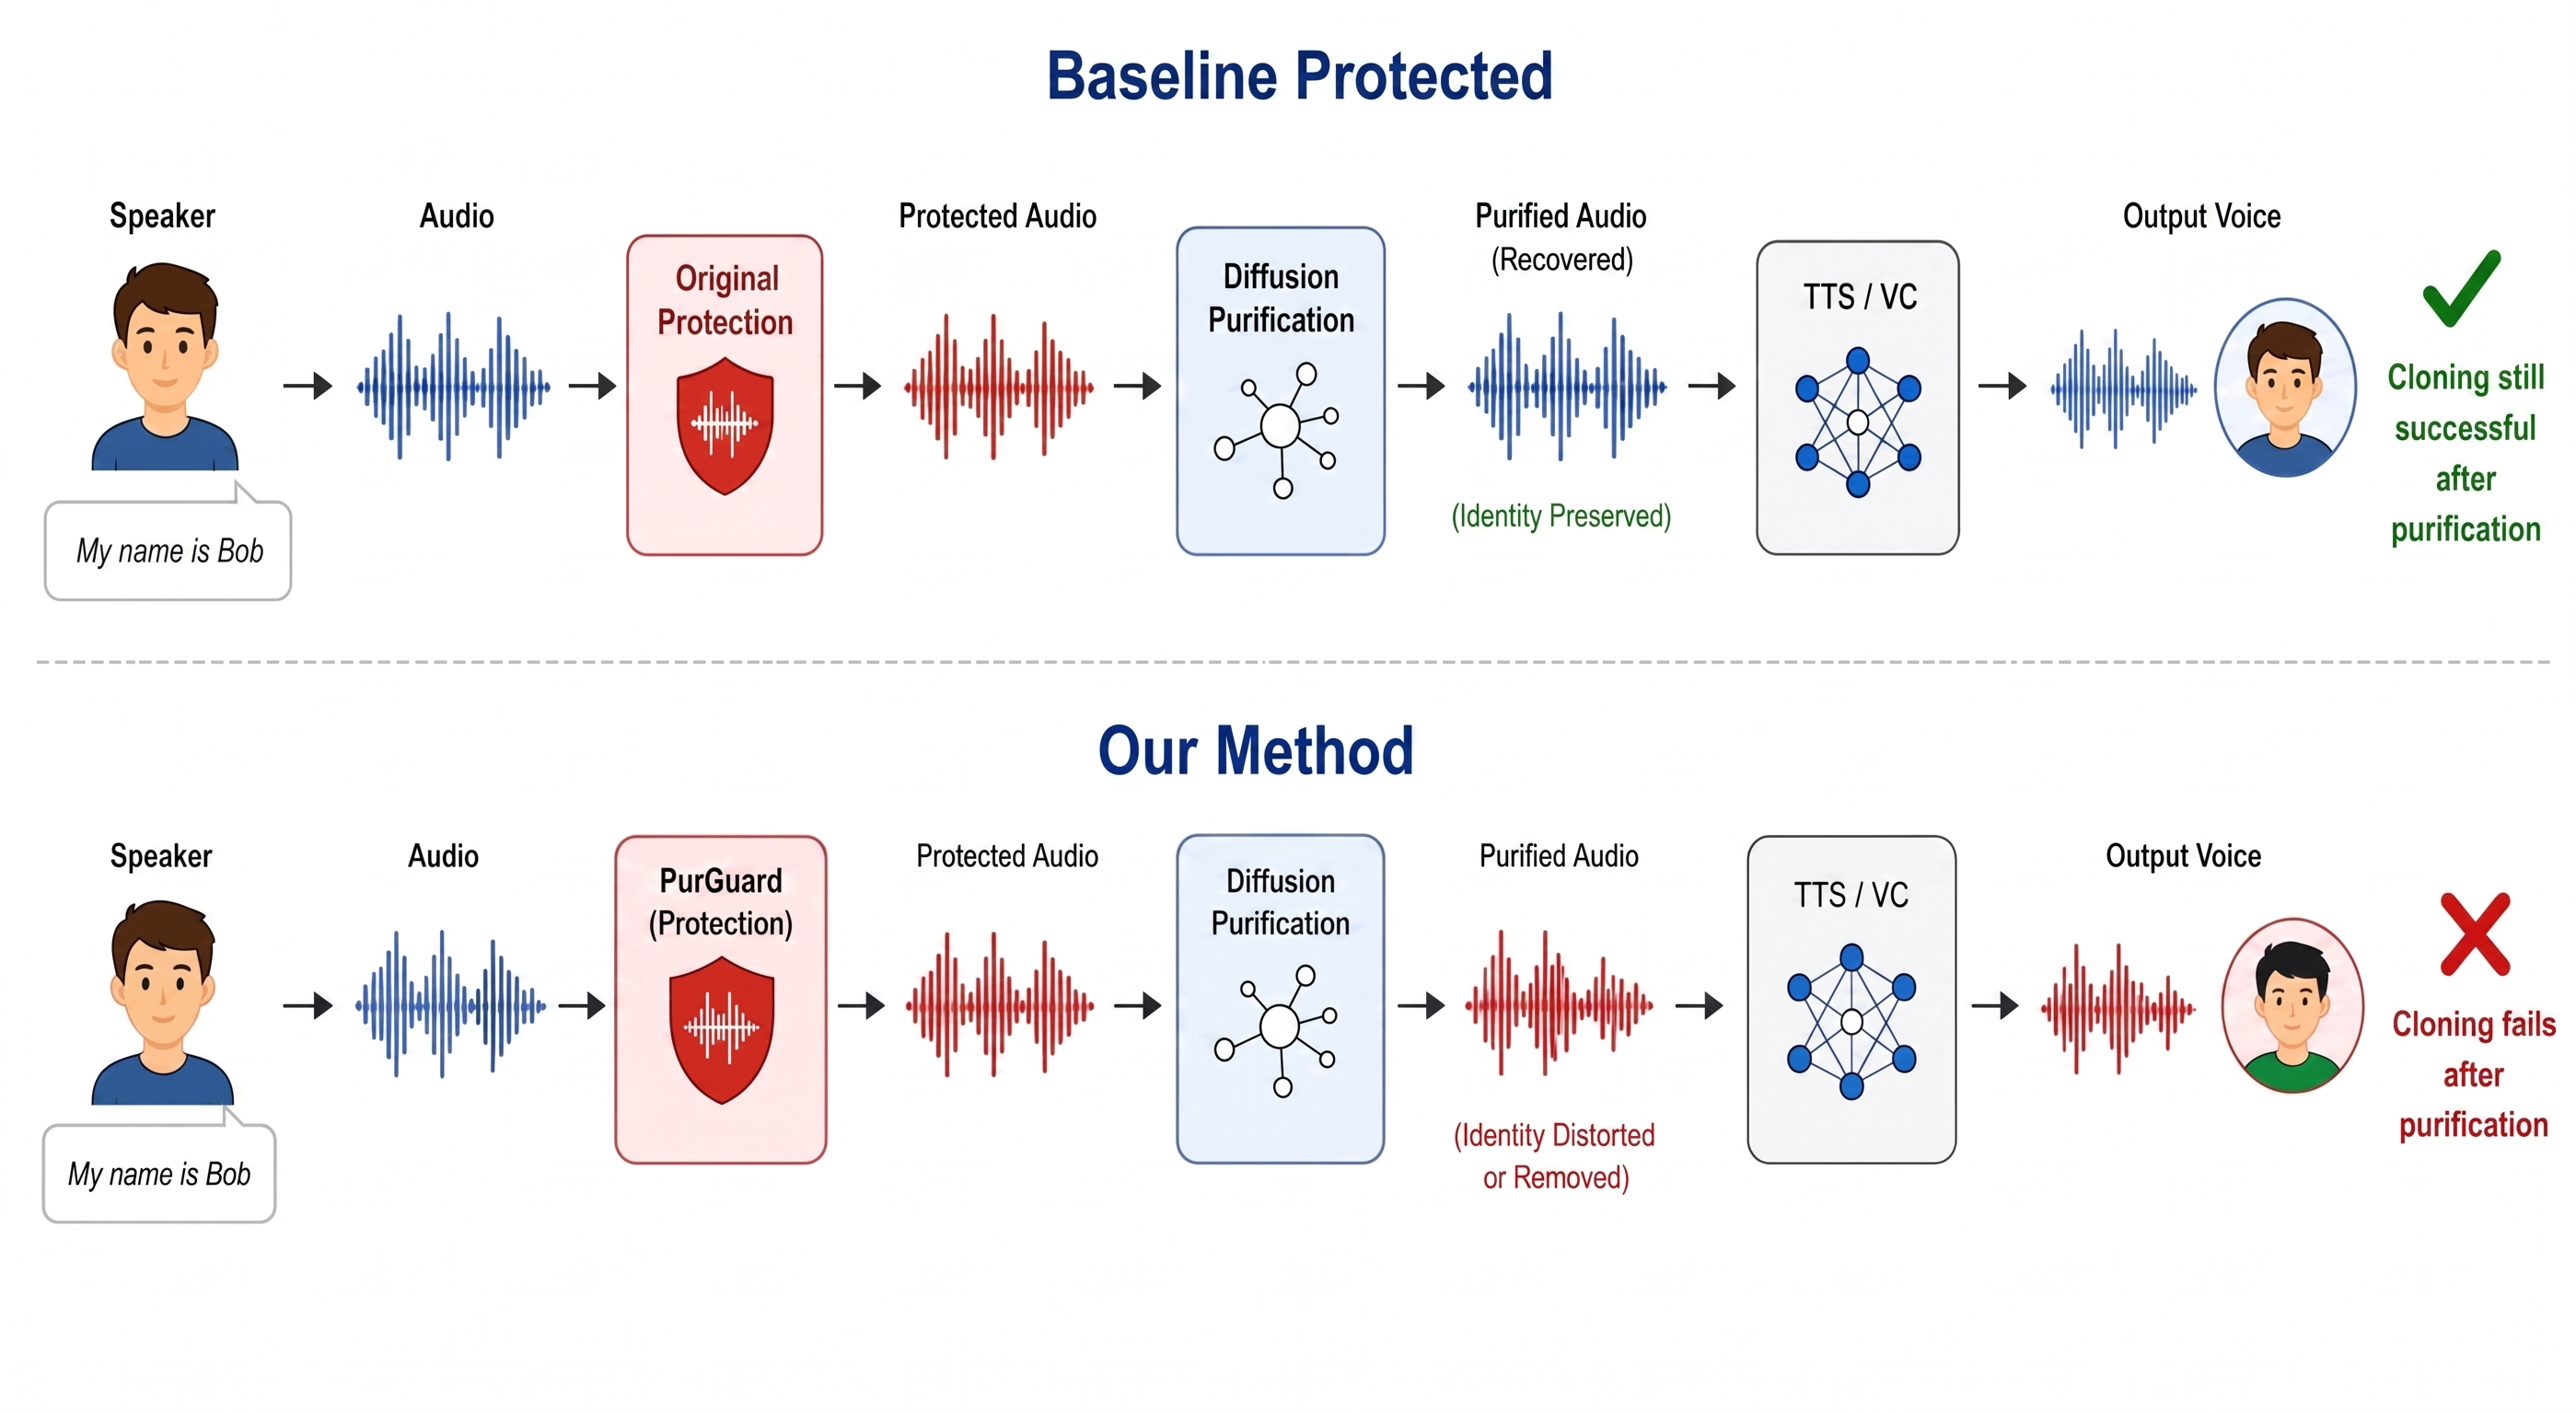
\includegraphics[width=\columnwidth]{Overview.png}
\caption{High-level attack chain for purification-aware voice protection: the defender releases protected speech, while the attacker applies a diffusion purifier before voice cloning.}
\label{fig:overview}
\end{figure}

Protective perturbation methods address this setting by adding small,
human-tolerable perturbations to the released waveform so that downstream voice cloning 
or speaker modeling systems extract unreliable identity information \cite{huang2021attackvc,li2023voiceguard,yu2023antifake,zhang2025safespeech,zhang2025e2evguard}. 
This line of work has advanced quickly: early methods attacked voice conversion or zero-shot cloning, while newer systems consider broader synthesis scenarios, stronger transferability, and perceptual constraints. 
Under a direct-cloning protocol, these defenses can make synthesized speech less similar to the source speaker.

The direct-cloning protocol, however, is no longer sufficient. 
We call the stronger threat a \emph{purification-removal attack}: after obtaining a protected public recording, the attacker first applies a diffusion purifier to remove protective perturbations and then feeds the recovered reference to a cloning backend. 
De-AntiFake and VocalBridge show that this purification stage can be inserted before cloning, 
using diffusion or bridge-diffusion models to remove protective perturbations and recover speaker-discriminative cues \cite{fan2024deantifake,abbasihafshejani2026vocalbridge}. 
In this attack chain, the attacker does not ask whether the protected waveform is immediately cloneable; the attacker first asks whether purification can convert it back into a useful reference. 
A defense that is optimized only for the unpurified input may therefore overstate user protection.

This paper studies the defender's side of the same arms race. The central gap is that existing voice protection methods usually treat purification as an external evaluation condition rather than as a differentiable adversary in the optimization loop. 
Meanwhile, DiffAttack shows that output-only supervision can be weak and proposes intermediate-step supervision over the diffusion trajectory, 
while DiffBreak shows that stochastic and adaptive evaluation can overturn apparent robustness claims for diffusion purification \cite{kang2024diffattack,kang2024diffbreak}. 
Voice anti-cloning is different: the target is a continuous speaker identity representation, the perturbation must remain suitable for public release, and the downstream misuse pipeline may contain unknown cloning backends.

We propose \method, a purification-aware framework for protective perturbation generation. Figure~\ref{fig:overview} summarizes the pipeline.
The key idea is simple: if the attacker depends on a purifier to recover speaker identity, 
then the defender should optimize the perturbation against the purifier, not only against the final cloning model. 
\method{} combines a speaker-disruption objective, which reduces similarity between the source speaker and the purified protected speech, 
with a trajectory-deviation objective, which pushes the reverse diffusion path away from its paired forward noising states. 
This makes purification resistance a training objective rather than an after-the-fact stress test.

Our implementation instantiates this idea with the first-stage DiffWave purifier from De-AntiFake, 
a differentiable ensemble of VITS, Tortoise, WavLM, and ECAPA-style speaker encoders when available, 
and independent ECAPA, x-vector, and Resemblyzer evaluators. 
We also define a purification-aware evaluation protocol with clean-purification controls, 
post-purification speaker similarity, thresholded speaker-verification acceptance, and quality metrics. 
The protocol is designed to answer the security question that matters in practice: whether protected speech remains non-cloneable after the attacker attempts to purify it.

Our contributions are:
\begin{itemize}
    \item We formulate \emph{purification-aware voice protection}, in which the defender must preserve speaker disruption even after an attacker applies diffusion-based perturbation removal.
    \item We introduce \method, a dual-objective optimization framework that jointly maximizes post-purification speaker-identity disruption and trajectory deviation inside the attacker's reverse diffusion process.
    \item We define a purification-aware evaluation protocol with clean-purification controls, calibrated speaker-verification thresholds, and repeated stochastic purification trials, 
    enabling fair comparison across protection methods and diffusion purifiers.
\end{itemize}

\section{Related Work}

\subsection{Proactive Voice Protection}

Proactive voice protection aims to modify speech before release so that unauthorized synthesis systems cannot reuse the speaker identity. 
AttackVC perturbs source speech to disrupt voice conversion \cite{huang2021attackvc}, 
VoiceGuard improves imperceptibility with time-domain constraints \cite{li2023voiceguard}, 
and AntiFake improves transferability by attacking speaker representations used by cloning systems \cite{yu2023antifake}. 
SafeSpeech expands the scenario to training-time malicious synthesis and emphasizes robust, universal perturbations \cite{zhang2025safespeech}. 
E2E-VGuard further considers end-to-end and LLM-based synthesis pipelines, where automatic transcription and timbre extraction jointly affect cloning quality \cite{zhang2025e2evguard}. 
These systems motivate our goal but share a common limitation: they optimize against the cloning or synthesis pipeline directly, 
and do not account for an attacker who first removes the perturbation with a diffusion purifier. 
\method addresses this gap by treating purification as a first-class component of the optimization target.

\subsection{Purification as an Adaptive Attacker}

Adversarial purification removes perturbations from the input before the downstream model consumes it. 
AudioPure shows that DiffWave-style forward noising followed by reverse denoising can defend audio recognition models against adversarial examples \cite{wu2023audiopure}. 
Later systems improve purification in different ways, including hierarchical diffusion \cite{guo2024wavepurifier}, efficient dual-domain purification \cite{tan2024dualpure}, 
and speaker-verification-oriented diffusion reconstruction \cite{bai2024dap}. 
These methods are valuable to an attacker in the voice anti-cloning setting because they can be used as a preprocessing step before synthesis.

De-AntiFake directly evaluates this risk for voice cloning and shows that purification can bypass several protective perturbation defenses \cite{fan2024deantifake}. 
VocalBridge strengthens this line by moving purification into a latent diffusion-bridge formulation that aims to recover clean, 
speaker-discriminative speech while avoiding transcript dependence \cite{abbasihafshejani2026vocalbridge}. 
These works expose the fragility of current protection methods under adaptive attackers. 
\method takes the complementary defender perspective: rather than building a stronger purifier, 
it generates perturbations that are optimized to resist purification, closing the loop between attack and defense.

\begin{figure*}[!t]
\centering
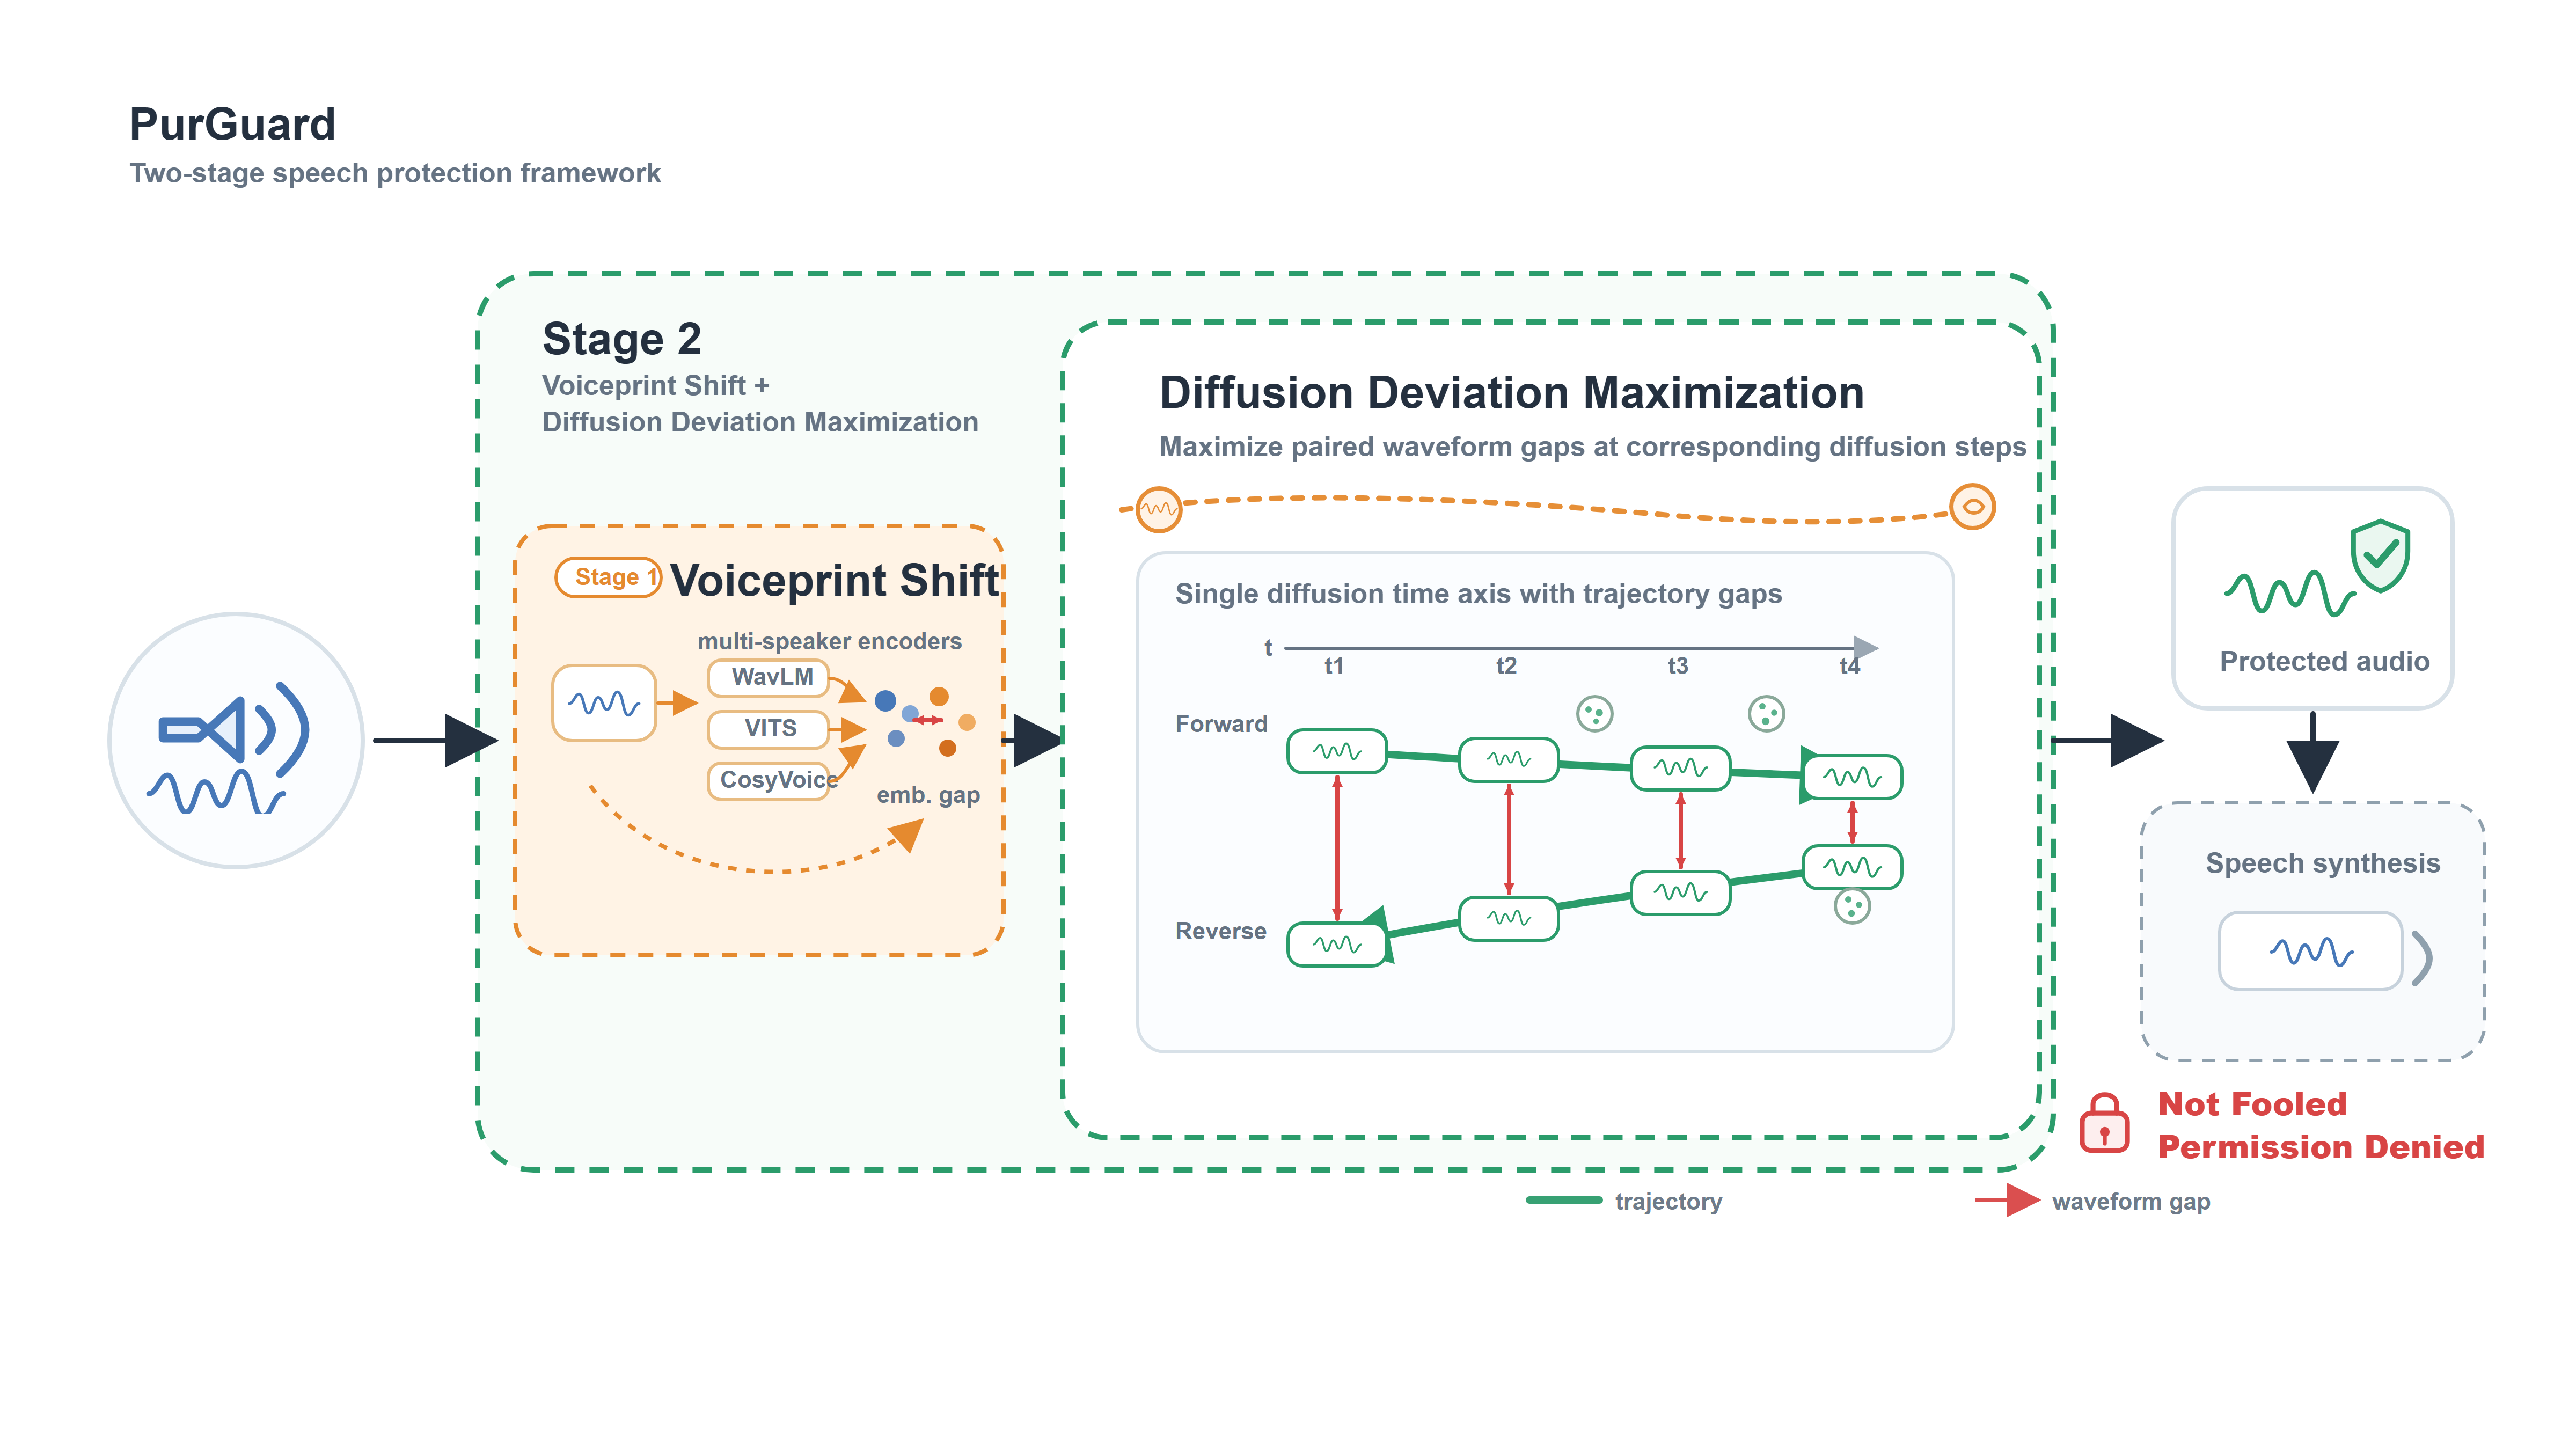
\includegraphics[width=\textwidth]{purguard-framework.png}
\caption{\method{} framework. The defender optimizes a bounded protective perturbation through a surrogate diffusion purifier, combining post-purification speaker-identity disruption with reverse-trajectory deviation so that purified protected speech remains unreliable for downstream cloning.}
\label{fig:purguard-framework}
\end{figure*}

\subsection{Adaptive Attacks on Diffusion Purification}

The conceptual foundation of \method is related to adaptive attacks on diffusion purification. 
DiffAttack shows that output-only supervision can be weak and proposes intermediate-step supervision over the diffusion trajectory \cite{kang2024diffattack}. 
DiffBreak further questions the apparent robustness of diffusion purification under stochastic and adaptive evaluation \cite{kang2024diffbreak}. 
These studies suggest two lessons for voice protection: the purifier's internal trajectory is an attack surface, and single-pass output evaluation can misrepresent robustness.

The closest naming and high-level conceptual overlap is AntiPure, which studies protective perturbations against diffusion-based purification for image customization \cite{yang2025antipure}. 
\method differs in domain and security objective: it protects released speech from post-purification voice cloning, measures failure in continuous speaker-embedding space, and must preserve perceptual audio quality while transferring across purifier, encoder, and cloning backends.

However, prior adaptive purification attacks differ from \method in three fundamental ways.
First, the \emph{optimization direction} is reversed: DiffAttack is an attacker's tool that causes a purified input to be misclassified, whereas \method is a defender's tool that causes a purified input to lose speaker identity before cloning.
Second, the \emph{perturbation constraint} is stricter in the voice setting: image perturbations need only be visually imperceptible, while voice perturbations must additionally satisfy perceptual audio quality bounds (PESQ, STOI) because the protected waveform is intended for public release and human listening.
Third, the \emph{success metric} is continuous rather than discrete: image robustness is measured by classification accuracy over a finite label set, whereas voice protection is measured by cosine similarity in a continuous speaker-embedding space, which produces denser gradient signals but requires the perturbation to suppress identity information across multiple independent encoder architectures.
These differences motivate a purpose-built trajectory-deviation objective for the voice domain, rather than a direct transfer of image-classification attack techniques.

\section{Method}

\subsection{Threat Model and Security Goal}

Figure~\ref{fig:purguard-framework} gives an overview of the \method{} framework. We study a proactive defense for public speech release. Let $x \in [-1,1]^T$ be a clean waveform from a protected speaker. The defender releases
\begin{equation}
    x_p = \mathrm{clip}_{[-1,1]}(x + \delta), \qquad \|\delta\|_{\infty} \leq \epsilon,
\end{equation}
where the perturbation budget keeps $x_p$ close to the original audio. The attacker wants to use the released audio as a reference for voice cloning, but first applies a diffusion-based purifier $\purifier$ to remove protective perturbations. The effective attack chain is therefore
\begin{equation}
    x_p \rightarrow \hat{x}=\purifier(x_p) \rightarrow \mathcal{C}(\hat{x}),
\end{equation}
where $\mathcal{C}$ is a downstream cloning or voice-conversion system.

The defender's goal is stronger than direct anti-cloning. A protected waveform should remain non-cloneable after the attacker purifies it. We call this property \emph{purification-resilient protection}: the purified protected reference $\purifier(x_p)$ should not preserve enough source-speaker information for successful cloning, while the protected waveform remains intelligible to human listeners.

We assume a strong white-box defender during perturbation generation. The defender has access to a surrogate purifier and can differentiate through its denoising process. This setting is not meant to assume that every deployed defender knows the attacker's exact purifier. Instead, it provides a worst-case design target: if a defense cannot survive a known purifier during optimization and evaluation, it is unlikely to survive adaptive purification attacks in practice.

In practice, the defender may not know which purifier the attacker will use. We address this in two ways. First, we evaluate transfer to held-out purifiers (AudioPure, DualPure, WavePurifier) that were not used during optimization, measuring how much protection degrades when the surrogate does not match the attacker's purifier. Second, the trajectory-deviation objective targets the structural behavior of diffusion reverse processes rather than the specific weights of one model, which we hypothesize improves cross-purifier transfer compared to output-only optimization. A fully black-box setting—where the defender has no access to any purifier during optimization—remains an open problem and is discussed in Section~\ref{sec:conclusion}.

\subsection{Design Rationale}

Existing voice protection methods typically optimize the released waveform against a cloning model or a speaker encoder. This direct objective can be effective when the attacker uses $x_p$ immediately. It becomes incomplete when the attacker first runs a purifier. In that setting, the important object is not only $x_p$, but the cleaned reference $\purifier(x_p)$ that the cloning system actually sees.

\method changes the defense target from the final cloning model to the full purification attack chain. The defense has two requirements. First, the purified audio should lose source-speaker identity according to speaker encoders that approximate cloning-relevant identity extraction. Second, the perturbation should interfere with the purifier's denoising process rather than behave like ordinary noise that the purifier can remove. These requirements lead to two complementary objectives: post-purification identity disruption and reverse-trajectory deviation.

\subsection{Purification-Aware Objective}

\method optimizes a bounded perturbation by solving
\begin{equation}
    \delta^{\star}
    = \arg\max_{\|\delta\|_{\infty}\leq\epsilon}
    \alpha \mathcal{L}_{\text{id}}(x_p;\purifier,\encoder)
    + \beta \mathcal{L}_{\text{traj}}(x_p;\purifier),
    \label{eq:overall_objective}
\end{equation}
where $\encoder=\{f_k\}_{k=1}^{K}$ is an ensemble of differentiable speaker encoders. The weights $\alpha$ and $\beta$ control the balance between identity disruption and purification resistance. Eq.~\eqref{eq:overall_objective} is the central methodological choice: purification is modeled as part of the adversary, not as a post-hoc evaluation step.

\subsection{Post-Purification Identity Disruption}

For each encoder $f_k$, let $e_k=f_k(x)$ be the source speaker embedding. In the untargeted setting, \method reduces source-speaker similarity after purification:
\begin{equation}
    \mathcal{L}_{\text{id}}
    =
    -\frac{1}{K}\sum_{k=1}^{K}
    \cos\!\left(f_k(\purifier(x_p)), e_k\right).
    \label{eq:identity_loss}
\end{equation}
This objective directly matches the attacker's use case. The attacker does not clone from the raw protected waveform; the attacker clones from the recovered reference $\purifier(x_p)$. Therefore, the identity objective is evaluated after purification.

The encoder ensemble reduces overfitting to one identity extractor. A single encoder can produce perturbations that exploit that encoder while transferring poorly to other cloning systems. Averaging over multiple encoders encourages perturbations that disrupt speaker information shared across common identity representations. Evaluation still uses held-out encoders, so success cannot be explained only by white-box access to the optimization ensemble.

\subsection{Reverse-Trajectory Deviation}

Optimizing only Eq.~\eqref{eq:identity_loss} can be weak because the gradient must pass through stochastic noising, multiple denoising steps, and a speaker encoder. More importantly, a final-output objective gives the purifier many opportunities to remove the perturbation before the identity loss is measured. \method therefore also constrains intermediate denoising behavior.

For a timestep $t$, define the paired forward noising state
\begin{equation}
    \begin{aligned}
    x_t^{+}
    &=
    \sqrt{\bar{\alpha}_t}x_p
    +
    \sqrt{1-\bar{\alpha}_t}z,\\
    z&\sim\mathcal{N}(0,I).
    \end{aligned}
\end{equation}
Starting from the terminal noisy state, the purifier produces reverse states $x_t^{-}$ along its denoising path. For captured timesteps $\mathcal{T}$, \method maximizes
\begin{equation}
    \mathcal{L}_{\text{traj}}
    =
    \frac{1}{|\mathcal{T}|}
    \sum_{t\in\mathcal{T}}
    \left\|x_t^{-}-x_t^{+}\right\|_2^2 .
    \label{eq:traj_loss}
\end{equation}

The role of Eq.~\eqref{eq:traj_loss} is not to make the waveform noisy. Its role is to make the purifier's intermediate reconstruction states disagree with the protected input's paired noising path. A purifier succeeds when its reverse process removes the perturbation while preserving the speaker cues needed for cloning. \method makes this process less reliable by pushing intermediate states away from the identity-preserving reconstruction path. This gives the perturbation a target inside the purifier, rather than relying only on the final purified waveform.

\subsection{Practical Optimization}

We use projected gradient ascent only as a solver for Eq.~\eqref{eq:overall_objective}. At iteration $i$,
\begin{equation}
    \begin{aligned}
    \tilde{x}_p^{(i+1)}
    &=
    \mathrm{clip}_{[-1,1]}
    \left(x_p^{(i)}+\eta\,\mathrm{sign}(\nabla_{x_p}\mathcal{L})\right),\\
    x_p^{(i+1)}
    &=\Pi_{x,\epsilon}\left(\tilde{x}_p^{(i+1)}\right),
    \end{aligned}
\end{equation}
where $\Pi_{x,\epsilon}$ projects to the $\ell_{\infty}$ ball around $x$. The algorithmic contribution is the purification-aware objective, not the use of projected gradient ascent.

The implementation differentiates through reverse steps separately and accumulates gradients, which avoids storing the full diffusion graph. The default pilot setting uses 16\,kHz mono audio, a 3\,s crop, $\epsilon=0.04$, $N=200$ optimization steps, $\eta=2\epsilon/N$, $\alpha=0.1$, and $\beta=0.9$. A staged schedule first optimizes direct identity disruption and then enables the purifier trajectory term. The current purifier is De-AntiFake's first-stage DiffWave model \cite{fan2024deantifake} with reverse timestep 5 and capture stride 1.

\subsection{Adaptive Adversary Discussion}

An adaptive attacker may change purification steps, random seeds, purifier architecture, or the downstream cloning backend. \method is designed to make this adaptation harder in three ways. First, the identity loss is measured after purification, so the defense targets the attacker's recovered reference rather than the raw protected audio. Second, the trajectory loss supervises intermediate states, which reduces dependence on a single final-output gradient. Third, the encoder ensemble and held-out evaluation separate the optimization models from the models used to judge cloning risk.

These choices do not make purification-resistant protection absolute. A sufficiently strong attacker could train a purifier against \method-generated examples, combine multiple purifiers, or use human-in-the-loop editing. We therefore evaluate \method as a robustness improvement under a stronger attack chain, not as a complete solution to voice impersonation. This framing matches the security goal of reducing the reliability of unauthorized cloning from public audio under realistic adaptive pressure.

\section{Evaluation}

\subsection{Research Questions}

The evaluation is organized around four questions.
\textbf{RQ1:} Do existing protective perturbations remain effective when an attacker purifies the released audio before cloning?
\textbf{RQ2:} Is speaker-only optimization sufficient, or does explicit trajectory supervision improve post-purification protection?
\textbf{RQ3:} Does protection transfer across diffusion and non-diffusion purifiers and independent speaker evaluators, rather than overfitting to one surrogate encoder?
\textbf{RQ4:} Does purification resistance come at an unacceptable perceptual-quality cost?

We evaluate on CMU-ARCTIC \cite{kominek2004cmuarctic}, using 18 speakers and sampling 100 utterances per speaker, for 1,800 utterances in total. 
We use CMU-ARCTIC because the attack chain studies reference-audio reuse for TTS and voice cloning: the corpus provides clean, transcript-aligned, multi-speaker recordings with enough utterances per speaker to support repeated purification and cloning trials under controlled conditions. 
Larger in-the-wild corpora such as VoxCeleb are complementary for demographic and channel-diversity studies, but they introduce uncontrolled recording conditions that can confound purifier and voice-cloning comparisons in this first benchmark. Following DiffBreak's finding that stochastic and adaptive evaluation can overturn apparent robustness claims for diffusion purification, 
all metrics are averaged over three independent purification seeds \cite{kassis2025diffbreak}.

\subsection{Compared Systems and Attack Chain}

\paragraph{Protection methods.}
The benchmark is designed to compare \textbf{AttackVC} \cite{huang2021attackvc}, \textbf{VoiceGuard} \cite{li2023voiceguard}, \textbf{AntiFake} \cite{yu2023antifake}, \textbf{SafeSpeech} \cite{zhang2025safespeech}, \textbf{E2E-VGuard} \cite{zhang2025e2evguard}, and \method. 
We treat all of them as proactive protection methods and evaluate how much source-speaker information remains after the attacker purifies and clones the protected reference. 
Internal variants of \method, including speaker-only, trajectory-only, and staged joint optimization, are used for ablation.

\paragraph{Purification front ends.}
The surrogate purifier used for optimization is the first-stage DiffWave model from \textbf{De-AntiFake} \cite{fan2025deantifake}. 
At evaluation time, we treat the attacker's target purifier as black-box to the defender and test transfer to \textbf{VocalBridge} \cite{abbasihafshejani2026vocalbridge}, \textbf{WavePurifier} \cite{guo2024wavepurifier}, \textbf{AudioPure} \cite{wu2023audiopure}, and \textbf{DualPure} \cite{tan2024dualpure}. 
These diffusion purifiers differ in representation, diffusion design, and reconstruction assumptions, making them useful black-box transfer tests for purification-aware protection.
To avoid limiting the threat model to diffusion-based removal, we also include non-diffusion signal-processing front ends. 
The non-diffusion suite follows transformations studied by SpeakerGuard for speaker-recognition robustness and WaveGuard for audio adversarial-example mitigation \cite{chen2023speakerguard,hussain2021waveguard}. 
Table~\ref{tab:traditional_purifiers} reports the traditional transformations used to test whether protection survives simpler attacker preprocessing such as smoothing, resampling, quantization, filtering, and mel-domain reconstruction.

\paragraph{Cloning backends and evaluators.}
After purification, the attacker uses the recovered reference in representative synthesis backends: CosyVoice, F5-TTS, Qwen3-TTS, and Chatterbox. 
Speaker similarity is measured by independent evaluators, including ECAPA-TDNN \cite{desplanques2020ecapa}, x-vector, and Resemblyzer/d-vector style encoders. 
This design separates the encoder used to optimize \method{} from the encoders used to evaluate protection.

\subsection{Main Reporting Template}

Table~\ref{tab:main_reporting_template} uses the same grouped layout commonly adopted in purification papers: each protection method is expanded by cloning backend, the \textbf{Protected} columns report the no-purification control, 
the purification groups report post-purification xSVA/dSVA under four diffusion-based removal attacks, and the rightmost \textbf{Total Avg.} pair is reserved for row-wise summaries. We omit SIM from this grouped template to keep the main comparison compact. Numerical cells are intentionally left as run outputs rather than hand-written claims, so the table can be populated directly from experiment logs.

\begin{table*}[t]
\centering
\scriptsize
\setlength{\tabcolsep}{2.1pt}
\renewcommand{\arraystretch}{1.08}
\newcommand{\theadpad}{\rule{0pt}{2.6ex}}
\newcommand{\metricpairmain}{\cellcolor{metricpink}\textbf{xSVA} & \cellcolor{metricblue}\textbf{dSVA}}
\newcommand{\mainmetrics}{-- & -- & -- & -- & -- & -- & -- & -- & -- & -- & -- & --}
\begin{tabular}{ll*{12}{c}}
\toprule
\multirow[b]{3}{*}{\shortstack[c]{Protection\\Method}}
& \multirow[b]{3}{*}{\shortstack[c]{VC/TTS\\Method}}
& \multicolumn{2}{c}{\multirow[b]{2}{*}{Protected}}
& \multicolumn{8}{c}{\theadpad Purification Method}
& \multicolumn{2}{c}{\theadpad Total} \\
\cmidrule(lr){5-12}
\cmidrule(lr){13-14}
& & \multicolumn{2}{c}{} &
\multicolumn{2}{c}{\theadpad AudioPure} &
\multicolumn{2}{c}{\theadpad DualPure} &
\multicolumn{2}{c}{\theadpad WavePurifier} &
\multicolumn{2}{c}{\theadpad De-AntiFake} &
\multicolumn{2}{c}{\theadpad Avg.} \\
\cmidrule(lr){3-4}
\cmidrule(lr){5-6}
\cmidrule(lr){7-8}
\cmidrule(lr){9-10}
\cmidrule(lr){11-12}
\cmidrule(lr){13-14}
& &
\theadpad\metricpairmain &
\metricpairmain &
\metricpairmain &
\metricpairmain &
\metricpairmain &
\metricpairmain \\
\midrule
\multirow{5}{*}{AntiFake}
& CosyVoice   & 0.00 & 10.00 & 0.00 & 16.78 & 0.00 & 0.33 & 0.00 & 0.11 & 0.00 & 19.56 & 0.00 & 9.36 \\
& F5-TTS      & 0.00 & 6.21 & 0.00 & 6.13 & 0.00 & 0.23 & 0.00 & 0.00 & 0.00 & 4.92 & 0.00 & 3.50 \\
& Qwen3-TTS   & 0.00 & 5.11 & 0.00 & 10.67 & 0.00 & 0.00 & 0.00 & 0.00 & 0.11 & 17.00 & 0.02 & 6.56 \\
& Chatterbox  & 0.00 & 5.33 & 0.00 & 12.00 & 0.00 & 0.11 & 0.00 & 0.11 & 0.11 & 19.67 & 0.02 & 7.44 \\
\rowcolor{avggray}
& \textbf{Avg.} & 0.00 & 6.66 & 0.00 & 11.39 & 0.00 & 0.17 & 0.00 & 0.06 & 0.06 & 15.29 & 0.01 & 6.71 \\
\midrule
\multirow{5}{*}{SafeSpeech}
& CosyVoice   & 0.00 & 13.89 & 0.00 & 14.00 & 0.00 & 0.00 & 0.00 & 0.11 & 0.00 & 20.00 & 0.00 & 9.60 \\
& F5-TTS      & 0.00 & 3.12 & 0.00 & 9.30 & 0.00 & 0.11 & 0.00 & 0.00 & 0.00 & 8.04 & 0.00 & 4.12 \\
& Qwen3-TTS   & 0.00 & 8.33 & 0.00 & 10.22 & 0.00 & 0.22 & 0.00 & 0.11 & 0.22 & 18.44 & 0.04 & 7.47 \\
& Chatterbox  & 0.00 & 7.67 & 0.00 & 8.00 & 0.00 & 0.00 & 0.00 & 0.22 & 0.33 & 19.69 & 0.07 & 7.12 \\
\rowcolor{avggray}
& \textbf{Avg.} & 0.00 & 8.25 & 0.00 & 10.38 & 0.00 & 0.08 & 0.00 & 0.11 & 0.14 & 16.54 & 0.03 & 7.07 \\
\midrule
\multirow{5}{*}{E2E-VGuard}
& CosyVoice   & \mainmetrics \\
& F5-TTS      & \mainmetrics \\
& Qwen3-TTS   & \mainmetrics \\
& Chatterbox  & \mainmetrics \\
\rowcolor{avggray}
& \textbf{Avg.} & \mainmetrics \\
\midrule
\multirow{5}{*}{AttackVC}
& CosyVoice   & \mainmetrics \\
& F5-TTS      & \mainmetrics \\
& Qwen3-TTS   & \mainmetrics \\
& Chatterbox  & \mainmetrics \\
\rowcolor{avggray}
& \textbf{Avg.} & \mainmetrics \\
\midrule
\multirow{5}{*}{VoiceGuard}
& CosyVoice   & \mainmetrics \\
& F5-TTS      & \mainmetrics \\
& Qwen3-TTS   & \mainmetrics \\
& Chatterbox  & \mainmetrics \\
\rowcolor{avggray}
& \textbf{Avg.} & \mainmetrics \\
\midrule
\multirow{5}{*}{\method}
& CosyVoice   & \mainmetrics \\
& F5-TTS      & \mainmetrics \\
& Qwen3-TTS   & \mainmetrics \\
& Chatterbox  & \mainmetrics \\
\rowcolor{avggray}
& \textbf{Avg.} & \mainmetrics \\
\midrule
\bottomrule
\end{tabular}
\caption{Main purification-aware benchmark in the grouped format used by prior purification work. Each metric pair reports xSVA/dSVA after cloning from the protected reference or the purified protected reference, and the rightmost Total Avg. pair is reserved for row-wise summaries. SIM is omitted here to keep the main table compact. Lower values indicate stronger retained protection from the defender's perspective. 
Results are to be populated from experiment logs for the protection methods listed at left, including \method.}
\label{tab:main_reporting_template}
\end{table*}

\subsection{Metrics and Controls}

The primary continuous metric is source-to-output speaker similarity:
\begin{equation}
    \mathrm{Sim}_{g,m}
    =
    \cos\!\left(g(x), g(\mathcal{C}_m(\purifier(x_p)))\right),
\end{equation}
where lower values indicate stronger retained protection. We also report speaker verification acceptance (SVA), attack success rate (ASR), post-purification protection rate (PPR), and quality metrics including SNR, PESQ, and STOI. 
Following De-AntiFake \cite{fan2025deantifake}, SVA is the average binary speaker-verification acceptance rate over cloned outputs:
\begin{equation}
    \mathrm{SVA}_{g,m,p}
    =
    \frac{1}{N}\sum_{i=1}^{N}
    \mathbb{I}\!\left[
        \cos\!\left(g(x_i), g(\mathcal{C}_m(p(x_{p,i})))\right)
        \ge \tau_g
    \right],
\end{equation}
where $g$ is the verification evaluator, $m$ is the cloning backend, $p$ is the purification setting, and $\tau_g$ is the calibrated acceptance threshold. 
In the full evaluation pipeline, \textbf{SIM} denotes the continuous source-to-output similarity under the primary ECAPA-TDNN evaluator. 
We report \textbf{xSVA} when $g$ is an x-vector verifier and \textbf{dSVA} when $g$ is a d-vector-style verifier; the main benchmark table omits SIM for compactness. 
Higher SIM, xSVA, or dSVA means the attacker more often recovers source-speaker identity; lower values mean stronger retained protection.
The most important controls are: clean reference, protected reference without purification, purified clean reference, and purified protected reference. 
The purified-clean control is essential because it verifies that a purifier preserves identity for benign inputs.

\subsection{Threshold Calibration}

The implementation includes calibrated decision thresholds for the independent speaker evaluators. 
Table~\ref{tab:thresholds} records the current calibration values used by the evaluation code. 
These thresholds convert continuous cosine similarity into verification-style acceptance and rejection rates.

\begin{table}[t]
\centering
\small
\begin{tabular}{lcc}
\toprule
Evaluator & EER & Threshold \\
\midrule
ECAPA-TDNN & 0.0037 & 0.3195 \\
x-vector & 0.0600 & 0.9472 \\
Resemblyzer & 0.0425 & 0.7235 \\
\bottomrule
\end{tabular}
\caption{Speaker-verification threshold calibration used by the current evaluation implementation. 
Thresholds are applied per evaluator when computing SVA and PPR.}
\label{tab:thresholds}
\end{table}

\subsection{Adaptive and Transfer Settings}

To distinguish robustness against a fixed diffusion purifier from robustness against an adaptive attack chain, we include three transfer settings. The first changes the purification front end while keeping the protected waveform fixed, covering both diffusion purifiers and non-diffusion transformations in Table~\ref{tab:traditional_purifiers}. 
The second changes the cloning backend after purification. The third changes the speaker verifier used to score the output. These tests measure whether \method{} overfits to the surrogate purifier or optimization encoders.

\begin{table*}[t]
\centering
\scriptsize
\setlength{\tabcolsep}{2.8pt}
\renewcommand{\arraystretch}{1.08}
\newcommand{\metricpair}{\cellcolor{metricpink}\textbf{SIM} & \cellcolor{metricblue}\textbf{WER}}
\begin{tabular}{lcccccccccccccccc}
\toprule
\multirow[b]{3}{*}{\shortstack[c]{Protection\\Method}}
& \multicolumn{8}{c}{SpeakerGuard~\cite{chen2023speakerguard}}
& \multicolumn{8}{c}{WaveGuard~\cite{hussain2021waveguard}} \\
\cmidrule(lr){2-9}
\cmidrule(lr){10-17}
& \multicolumn{2}{c}{RS}
& \multicolumn{2}{c}{Mel}
& \multicolumn{2}{c}{QD}
& \multicolumn{2}{c}{FL}
& \multicolumn{2}{c}{RS}
& \multicolumn{2}{c}{LPC}
& \multicolumn{2}{c}{QD}
& \multicolumn{2}{c}{NR} \\
\cmidrule(lr){2-3}
\cmidrule(lr){4-5}
\cmidrule(lr){6-7}
\cmidrule(lr){8-9}
\cmidrule(lr){10-11}
\cmidrule(lr){12-13}
\cmidrule(lr){14-15}
\cmidrule(lr){16-17}
& \metricpair
& \metricpair
& \metricpair
& \metricpair
& \metricpair
& \metricpair
& \metricpair
& \metricpair \\
\midrule
AntiFake & -- & -- & -- & -- & -- & -- & -- & -- & -- & -- & -- & -- & -- & -- & -- & -- \\
SafeSpeech & -- & -- & -- & -- & -- & -- & -- & -- & -- & -- & -- & -- & -- & -- & -- & -- \\
E2E-VGuard & -- & -- & -- & -- & -- & -- & -- & -- & -- & -- & -- & -- & -- & -- & -- & -- \\
AttackVC & -- & -- & -- & -- & -- & -- & -- & -- & -- & -- & -- & -- & -- & -- & -- & -- \\
VoiceGuard & -- & -- & -- & -- & -- & -- & -- & -- & -- & -- & -- & -- & -- & -- & -- & -- \\
\method{} & -- & -- & -- & -- & -- & -- & -- & -- & -- & -- & -- & -- & -- & -- & -- & -- \\
\bottomrule
\end{tabular}
\caption{Non-diffusion purification-front-end reporting template. 
SpeakerGuard transformations cover randomized smoothing (RS), mel-spectrogram reconstruction (Mel), quantization--dequantization (QD), and filtering (FL); WaveGuard transformations cover resampling (RS), linear predictive coding (LPC), quantization--dequantization (QD), and noise reduction (NR). 
Each setting reports speaker similarity (SIM) and word error rate (WER), testing whether lightweight signal-processing transformations weaken protection without a learned diffusion purifier.}
\label{tab:traditional_purifiers}
\end{table*}

We also evaluate stochastic purification by varying random seeds and reporting either mean performance with dispersion or worst-case performance across seeds. This is necessary because a defense may look successful under one denoising sample while failing under another. 
Finally, we include the purified-clean control for every purifier. If a purifier damages clean speech identity, then poor cloning after purification cannot be credited to the protection method.

\subsection{Ablations and Robustness Analyses}

The core ablation compares three variants: \textbf{Speaker-only}, which removes $\mathcal{L}_{\text{traj}}$; \textbf{Trajectory-only}, which removes the post-purification identity term; and \textbf{\method{}}, which uses both terms.
A second ablation varies $\alpha$ and $\beta$ to measure the trade-off between direct identity disruption and purification resistance. 
A third ablation varies the reverse timestep and capture stride to test whether robustness depends on a narrow diffusion schedule.

Because DiffBreak shows that stochastic and adaptive evaluation can overturn apparent robustness claims for diffusion purification, we report repeated purification samples or worst-case statistics over seeds \cite{kassis2025diffbreak}. 
We pair identity metrics with SNR, PESQ, and STOI so that improvements cannot be attributed merely to excessive audible distortion. 
Together, these experiments test the main claim of \method{}: once purification becomes part of the attack chain, robust voice protection should be optimized against the purifier itself.

\subsection{Artifact and Reproducibility Plan}

For reproducibility, we release perturbation-generation code, purifier wrappers, evaluation scripts, threshold-calibration code, configuration files, random seeds, and metadata for all generated protected samples. 
The artifact separates protected audio, purified audio, and cloned outputs so that each stage can be audited for identity loss. 
Because the work involves voice identity and impersonation risk, released audio follows dataset licenses and avoids examples that identify private speakers.


\section{Limitations}
\label{sec:limitations}
\method{} currently studies surrogate-based purification-aware optimization and evaluates whether the resulting protection transfers to black-box target purifiers. 
This captures the practical case where the defender can train against a local purifier but does not know the attacker's deployed purifier; it does not fully cover no-surrogate defenders, learned purifier ensembles, or attackers who jointly adapt purification and synthesis. 
The current implementation also focuses on waveform-domain perturbations with bounded amplitude; future work should add psychoacoustic masking, over-the-air transformations, and human listening studies. 
We do not adversarially train a new purifier on \method-generated samples; the current held-out purifier, seed, backend, and verifier transfer tests are a bounded proxy for adaptive attackers, not a full solution to iterative attack-defense retraining.
We plan to extend the benchmark with broader stochastic purification trials before drawing claims across all purifiers and cloning backends.

\section{Conclusion}
\label{sec:conclusion}

\method{} reframes voice anti-cloning as a purification-aware protection problem. 
Instead of assuming that a protected waveform is fed directly into a cloning system, we model the stronger and increasingly realistic attacker who first removes perturbations with a purification front end. 
For diffusion purifiers, protection must survive not only direct speaker extraction but also the attacker's reverse denoising path; 
for traditional signal-processing front ends, it must also survive lightweight transformations such as resampling, quantization, filtering, and denoising.

\method{} addresses this gap by combining pre-purification speaker disruption, post-purification speaker disruption, and trajectory-level deviation inside the purifier, 
and by providing a benchmark protocol with clean-purification controls and calibrated evaluator thresholds. 
The planned ablations are designed to test whether trajectory supervision is a necessary complement to pre- and post-purification identity optimization, and whether output-level gradients alone fail under stochastic purification.

The broader implication is that voice protection should be evaluated as part of an adaptive purification-and-cloning chain, not only as a direct perturbation against a cloning backend. 
We plan to provide an anonymized implementation and evaluation protocol to support reproducible review of this problem.


\section{Ethical Considerations}
This work studies defenses against unauthorized voice cloning and therefore involves dual-use capabilities. The intended use of \method{} is to help speakers publish audio with reduced risk of impersonation after purification-based removal attacks. 
The evaluation uses CMU-ARCTIC, a public speech corpus, and reports aggregate metrics rather than speaker-identifying examples. 
Released artifacts will exclude cloned outputs that could be reused for impersonation or provide them only through controlled review channels with clear use restrictions. 
We do not claim that perturbation-based protection replaces policy, watermarking, authentication, or platform-side abuse detection; 
rather, it provides a data-source defense that can be combined with these safeguards.

\section{LLM Usage Statement}
Large language models were used as writing assistants for organization, editing, and wording suggestions. 
All technical claims, citations, experiments, and final text remain the responsibility of the authors.

\bibliographystyle{IEEEtran}
\bibliography{custom}

\end{document}
